\chapter{Projekt systemu}
\thispagestyle{chapterBeginStyle}

    W tej części opisane zostały wymagania dla aplikacji w kontekście możliwości interakcji przez
użytkownika.



\section{Wymagania aplikacji}
\begin{enumerate}
    \item Użytkownik może wybrać jedną z predefiniowanych paczek łamigłówek by przejść do wyboru łamigłówki
    \item Użytkownik może wybrać jedną z predefiniowanych łamigłówek w paczce by przejść do jej rozwiązywania
    \item Użytkownik może rozwiązać łamigłówkę przy użyciu wyświetlanej planszy
    \item Użytkownik może oznaczać pola, co do których ma pewność, że są puste
    \item Aplikacja śledzi błędy użytkownika w trakcie rozwiązywania łamigłówki i przerywa jej rozwiązywanie
w przypadku popełnienia zbyt wielu błędów
    \item Postęp rozwiązywania łamigłówki jest zapisywany przy wyjściu do poprzedniego ekranu
    \item W menu wyboru łamigłówki wyświetlany jest stan łamigłówki tak, by można było ocenić:
    \begin{itemize}
        \item czy została rozpoczęta
        \item czy została ukończona bez przegranej
        \item czy została ukończona z przegraną
    \end{itemize}
    \item Użytkownik może wprowadzić łamigłówkę dla solvera za pomocą ekranu wprowadzania łamigłówki
    \item Użytkownik może wybrać łamigłówkę do rozwiązania dla solvera
    \item Użytkownik może nakazać rozwiązanie wprowadzonej łamigłówki
\end{enumerate}



\section{Nawigacja pomiędzy aktywnościami}
    Aplikacja otwiera się w menu głównym. W menu głównym dostępne są dwie zakładki: zakłada użytkownika
i zakładka w solvera. W zakładce użytkownika, użytkownik najpierw wybiera paczkę łamigłówek, a
następnie łamigłówkę do rozwiązania, po czym przechodzi do ekranu rozwiązywania. W zakładce solvera
dostępna jest lista wprowadzonych i predefiniowanych łamigłówek dla solvera. Użytkownik może przejść
do ekranu wprowadzania łamigłówki, by dodać kolejną łamigłówkę, bądź do ekranu auto-rozwiązywania,
gdzie nakazuje solverowi rozwiązanie wprowadzonej łamigłówki.

    Zależności między opisanymi aktywnościami są ukazane na diagramie.

\begin{figure}[!htb]
    \centering
    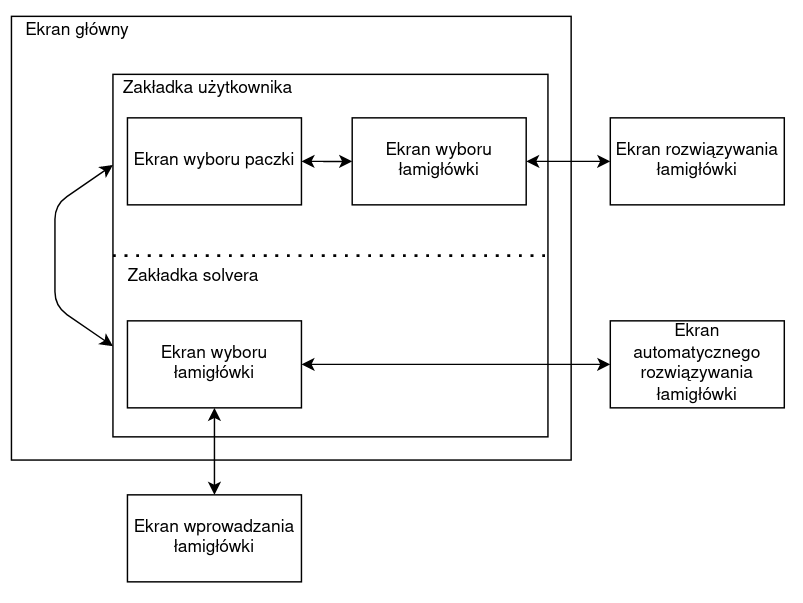
\includegraphics[width=\textwidth]{images/screens_diagram.png}
    \caption{Diagram zależności między aktywnościami}
    \label{diagAktywnosci}
\end{figure}
